%-------------------------------------------------------------------------------
\section{Introduction}
%-------------------------------------------------------------------------------
Web applications today own, store, and manage user data~\cite{nytimes:fb, npr:data}. 
This places a great responsibility on application developers to enforce the data protection rights
of users, through protecting users' rights to privacy and by moderating data content.
%
Recent developments have renewed efforts to improve the state of data protection in web
applications, creating incentives to support different forms of \emph{data protection
transformations}. 

One such transformation performs privacy-preserving user unsubscription from a service, as mandated
by laws such as the EU's General Data Protection Regulation (GDPR)~\cite{eu:gdpr} and California's
Consumer Privacy Act (CCPA)~\cite{ca:privacy-act} that codify users' rights to data ownership and
right to be forgotten.  Unsubscription motivates a need for an identify-revealing resubscription
transformation, making it easy for users to return instead of forcing users to permanently give up
their accounts.

Another such transformation anonymizes stale or inactive users' data, 
incentivized by the requirement to keep as little identifying information as possible
around that could compromise users, and prevent the data leaks that have led of the loss of livelihoods and
lawsuits~\cite{breach:amazon,breach:twitter, breach:fb, breach:marriott, breach:quora}, .

Finally, applications increasingly perform content moderation of harmful, plagiarised, or protected
data, which requires web applications to transform data contents~\cite{contentmod, sasb}.

Achieving these various data protection transformations is not easy.  For example, applications must
selectively retain unsubscribing users' data for legal or application purposes while properly
de-identifying this data, a non-trivial task in the face of subtle inference attacks.  Because these
transformations are necessarily application-specific and require handling complex data correlations,
today's applications often lack support for these transformations, or use ad-hoc methods to achieve
them, often with unclear guarantees.

To help developers of new and existing applications support data privacy transformations, we propose
\sys, which makes the key insight to model application data as an abstract \emph{entity graph}, and
represent data protection transformations as transformations of this graph. \emph{Ghost entities}
allow transformations to achieve both data retention and de-identification, and declarative
\emph{ghost policies} specify (reversible) transformations to the graph.

With \sys, developers specify a declarative, high-level data transformation policy by choosing from
a menu of provided edge and node transformations. This policy specifies the post-transformation
state of any instance of the entity graph. When the policy is invoked, \sys automatically and
systematically applies these transformations to the current entity graph instance according to the
policy.

We evaluate a prototype design and implementation for \sys, finding that \sys performs automatic
data protection transformations efficiently, and that policies can be expressed with low burden for
application developers.

\iffalse
%\begin{figure*}[ht!]
%    \centering
%    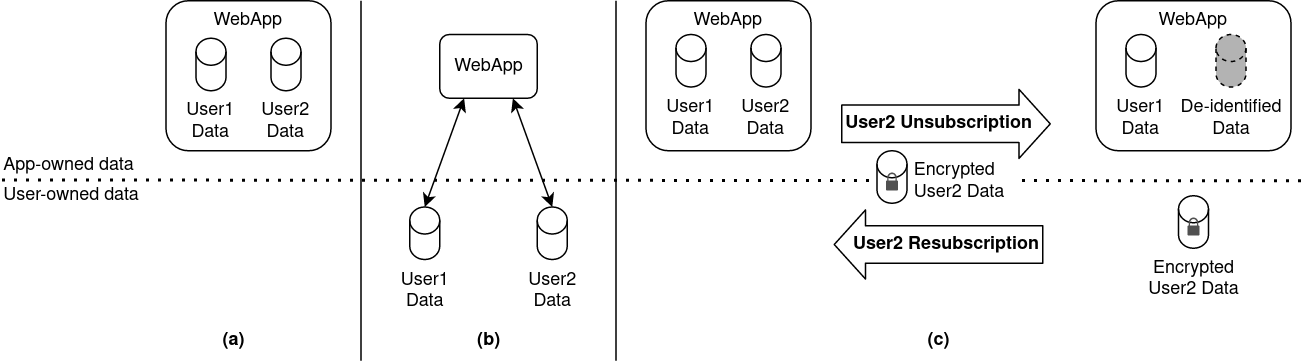
\includegraphics[width=\textwidth]{img/worlds}
%
%    \caption{\textbf{(a)} The current web application paradigm, in which applications maintain and
%    own user data; \textbf{(b)} A paradigm that decouples user data from web applications, giving users ownership of their data;
%    \textbf{(c)} \name, which allows users to switch between privacy-preserving unsubscribed mode (right) and identity-revealing subscribed mode (left).}
%    \label{fig:world}
%\end{figure*}
%
Web applications today own, store, and sell user data, often without the user's knowledge or
explicit consent~\cite{nytimes:fb, npr:data}. This both violates users' right for privacy, and has
dangerous consequences for both users and application developers as data leaks lead to loss of
livelihoods and lawsuits~\cite{breach:amazon,breach:twitter, breach:fb, breach:marriott,
breach:quora}. 
%Granting web applications complete ownership of personal data clearly fails to
%protect users' privacy. 

Although users want stronger privacy, completely decoupling user data from applications results in a
potentially even less desirable world. While possible~\cite{solid, amber, w5, blockstack, bstore}, such a
model hinders service-side computation and application performance, and requires users to manage
long-time security and storage of their data, leading to a lack of adoption in practice (Section~\ref{sec:related}).  

This paper proposes \name, a new paradigm that grants users flexible privacy when using web
applications, balancing users' desire for privacy with their desire for application utility. In
\name, users subscribe to applications by granting a time-limited lease to their data, with the
provision that the application may retain only de-identified information once the user unsubscribes.
Users flexibly switch between a privacy-preserving unsubscribed mode and an identity-revealing
subscribed mode at any time without permanently losing their data. \name contrasts
with the current web application paradigm for data ownership, in which applications have complete
ownership, and the other extreme in which the user has complete data ownership.% (see Figure~\ref{fig:world}). 

\name benefits users: they can choose privacy at any time, without
permanently losing their accounts or affecting the utility of the applications for others.  Just as
importantly, \name also benefits application developers. Recent laws such as the
European Union's General Data Protection Regulation (GDPR)~\cite{eu:gdpr} and California's Consumer
Privacy Act (CCPA)~\cite{ca:privacy-act} codify users' rights to data ownership, granting users the
right to request erasure of information related to them. Supporting \name enables
applications to comply with these legal mandates, while still allowing its departing users to easily
come back: if applications must let users leave, it is in their best interest to make it easy for
them to return.  

Furthermore, applications can continue to operate using their current revenue model, maintaining
performance, reliability, and utility for their users.  Because applications retain use of
subscribed users' data, and de-identified data of unsubscribed users, applications optimize the
amount of data available to generate profit and provide utility for subscribed users. The
application holds only identifying data for subscribed users, reducing the amount of
compromising data in the system to only those users who have actively agreed to temporarily give up
their privacy.

Realizing \name poses a number of technical challenges.
Unsubscription and resubscription requires complex and fragile data transformations: developers must
selectively retain unsubscribed users' data for legal or application purposes while properly
de-identifying this data, a non-trivial task in the face of subtle inference attacks (\eg tags on a
user's post can identify the user). De-identification and data removal needs to be reversible,
allowing the user to resubscribe at any time to their last-known subscribed state.

To make \name a reality, we model application data as an abstract \emph{entity graph}, and
represent unsubscription and resubscription as transformations of this graph.
\emph{Ghost entities} allow transformations to achieve both data retention and de-identification,
and declarative \emph{ghost policies} specify reversible transformations upon unsubscription.
We design and implement \sys, a practical system that systematically automates this transformation for new and existing applications, helping developers realize the \name paradigm without onerous labor.
%that takes a developer-specified unsubscription policy for the application's entity
%graph, and ensures that 
%that requires developers only to specify an abstract unsubscription policy on the 
%helps developers of databased-backed web applications automatically achieve correct, privacy-compliant user unsubscription and
%resubscription without onerous labor.
\fi
